\documentclass{article}
\usepackage[utf8]{inputenc}
\usepackage{graphicx}
\usepackage{fancyhdr}
\pagestyle{fancyplain}
\author{Mikkel, Jannik, Rune \& Rasmus}
\date{\today}
\lhead{Mikkel, Jannik, Rune \& Rasmus}
\rhead{\today}
\begin{document}

\section{Eksperimentdesign}

\subsection{Tidsmåling}

\subsection{Realisme}


\subsection{Andre Parametre}

\subsection{Tese}

\section{Implementation}

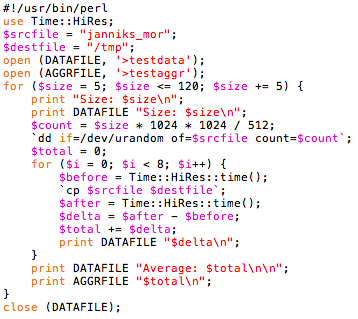
\includegraphics[width=4in]{kode.png}

\subsection{Omstændigheder}

\subsection{Graf}

\begin{figure}
	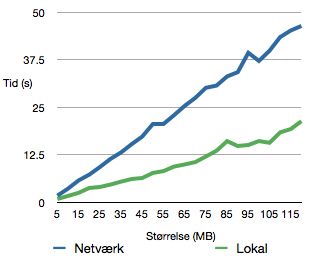
\includegraphics[width=4in]{ploto.png}
	\caption{Hej}
	\label{ploto}
\end{figure}

\begin{figure}
	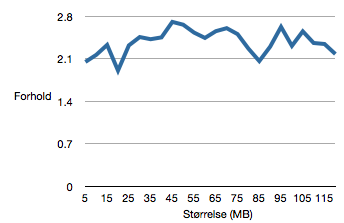
\includegraphics[width=4in]{plotforhold.png}
	\caption{Hej}
	\label{plotforhold}
\end{figure}

\subsection{Teseoverlevelse}

\subsubsection{i}

\subsubsection{ii}

\section{Ræssonnering}

\subsection{a}
\subsection{b}
\subsection{c}

\section{4...}

\end{document}
